% \begin{document}

\chapter{Teoria dei grafi}

Riferimento principale: Stanley, \textit{Algebraic Combinatorics}.

\section{Introduzione}

\dfn{Grafo}{\label{def:grafo}
  Un \textit{grafo} $ G $ e' la terna $ (V, E, \varphi) $ dove $ V $ e' un insieme finito di \textit{vertici}, $ E $ e' un insieme finito di \textit{lati} e
  \[
    \varphi : E \longrightarrow \left(\!\!\binom{V}{2}\!\!\right)
  \]
  associa ad ogni lato la coppia (non ordinata) di vertici ad esso adiacenti. Qui $ \left(\!\!\binom{V}{2}\!\!\right) $ denota il \textit{multi-insieme} di taglia $ 2 $ su $ V $: ammettiamo cioe' anche coppie del tipo $ \{v, v\} $ (\textit{loop}). Tutti i grafi che consideriamo sono \textbf{non orientati}.
}

\ex{}{
  Per $ V = \{v_1, v_2, v_3\} $ con lati $ e_1, e_2, e_3 $ e $ \varphi(e_1) = \{v_1, v_2\} $: scriveremo brevemente $ \varphi(e_1) = v_1 v_2 $.
}

\dfn{Lato multiplo}{\label{def:lato-multiplo}
  Se esistono lati distinti $ e_1, \ldots, e_k \in E $ con
  \[
    \varphi(e_1) = \cdots = \varphi(e_k) = uv ,
  \]
  diciamo che fra $ u $ e $ v $ c'e' un \textit{lato multiplo}.
}

\dfn{Grafo semplice}{\label{def:grafo-semplice}
  Un grafo $ G $ si dice \textit{semplice} se non ha loops ne' lati multipli: equivalentemente, $ \varphi $ e' iniettiva e a valori in $ \binom{V}{2} $ (coppie distinte, senza ripetizione), ossia
  \[
    E \subseteq \binom{V}{2} .
  \]
}

\subsection{Matrice di adiacenza e conteggio cammini}

\subsubsection{La matrice $ A(G) $}

\dfn{Matrice di adiacenza}{\label{def:matrice-adiacenza}
  Sia $ G $ un grafo con vertici $ V = \{v_1, \ldots, v_p\} $. La \textit{matrice di adiacenza} $ A(G) \in \mathbb{N}^{p \times p} $ ha entrate
  \[
    A(G)_{ij} := \#\{\text{lati incidenti a } v_i \text{ e a } v_j\} .
  \]
}

Proprieta' immediate:
\begin{itemize}
  \item $ A(G) $ e' \textbf{simmetrica} (i grafi non sono orientati);
  \item la traccia $ \mathrm{Tr}(A(G)) = \sum_i A(G)_{ii} $ conta il numero di \textit{loops};
  \item essendo simmetrica reale, $ A(G) $ e' \textbf{diagonalizzabile} (teorema spettrale).
\end{itemize}

\ex{}{
  Per il grafo su $ \{v_1, \ldots, v_5\} $ con due loop su $ v_3 $, un loop su $ v_4 $, un loop su $ v_5 $, lato doppio fra $ v_1 $ e $ v_2 $, lati semplici $ v_1 v_3 $, $ v_1 v_4 $, $ v_2 v_5 $, $ v_3 v_5 $:
  \begin{center}
    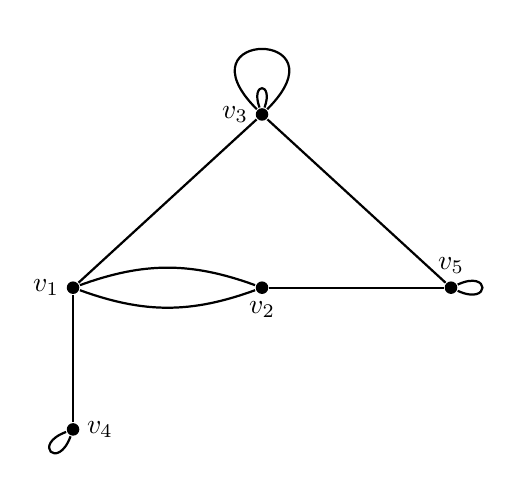
\begin{tikzpicture}[
      vertex/.style={circle, fill=black, inner sep=1.6pt},
      every label/.style={inner sep=2pt},
      thick
    ]
      \node[vertex, label=left:$v_3$]  (v3) at (0, 2.2) {};
      \node[vertex, label=left:$v_1$]  (v1) at (-2.4, 0) {};
      \node[vertex, label=below:$v_2$] (v2) at (0, 0) {};
      \node[vertex, label=above:$v_5$] (v5) at (2.4, 0) {};
      \node[vertex, label=right:$v_4$] (v4) at (-2.4, -1.8) {};

      % Lato doppio v_1--v_2
      \draw (v1) to[bend left=20] (v2);
      \draw (v1) to[bend right=20] (v2);
      % Lati semplici
      \draw (v1) -- (v3);
      \draw (v1) -- (v4);
      \draw (v2) -- (v5);
      \draw (v3) -- (v5);

      % Loops
      \draw (v3) to[out=70, in=110, looseness=14] (v3);
      \draw (v3) to[out=45, in=135, looseness=28] (v3);
      \draw (v4) to[out=200, in=250, looseness=15] (v4);
      \draw (v5) to[out=-25, in=25, looseness=15] (v5);
    \end{tikzpicture}
  \end{center}
  La matrice di adiacenza e':
  \[
    A(G) = \begin{pmatrix}
      0 & 2 & 1 & 1 & 0 \\
      2 & 0 & 0 & 0 & 1 \\
      1 & 0 & 2 & 0 & 1 \\
      1 & 0 & 0 & 1 & 0 \\
      0 & 1 & 1 & 0 & 1
    \end{pmatrix} .
  \]
  Traccia $ 0 + 0 + 2 + 1 + 1 = 4 $: ci sono in tutto $ 4 $ loop nel grafo.
}

Vedremo come autovalori di $ A(G) $ e cammini sul grafo siano strettamente collegati.

\subsubsection{Potenze di $ A(G) $ e cammini}

\dfn{Cammino}{\label{def:cammino}
  Un \textit{cammino} di lunghezza $ \ell $ da $ u $ a $ v $ in $ G $ e' una sequenza
  \[
    v_1\, e_1\, v_2\, e_2\, \cdots\, e_\ell\, v_{\ell+1}
  \]
  con $ v_1 = u $, $ v_{\ell+1} = v $ e $ \varphi(e_i) = v_i v_{i+1} $ per ogni $ i $.
}

\nt{
  Invertire l'ordine di un cammino da' un cammino fra gli stessi due vertici, di stessa lunghezza.
}

\thm{Potenze della matrice di adiacenza}{\label{thm:potenze-A}
  Per ogni $ \ell \in \mathbb{Z}_{\geq 1} $:
  \[
    \bigl(A(G)^\ell\bigr)_{ij} = \#\{\text{cammini di lunghezza } \ell \text{ da } v_i \text{ a } v_j\} .
  \]
}
\nt{
  E' lo stesso principio delle \textit{catene di Markov}: le potenze della matrice di transizione contano le traiettorie di lunghezza fissata.
}
\pf{Dim}{
  Conseguenza diretta della definizione di prodotto di matrici. Posto $ A := A(G) $ con entrate $ a_{rs} $, e detto $ p = |V| $ il numero di vertici di $ G $:
  \[
    \bigl(A^\ell\bigr)_{ij}
      = \sum_{i_1, \ldots, i_{\ell-1} = 1}^{p} a_{i, i_1}\, a_{i_1, i_2}\, \cdots\, a_{i_{\ell-1}, j}\,.
  \]
  Fissata la sequenza di indici intermedi $ (i_1, \ldots, i_{\ell-1}) $, il prodotto $ a_{i, i_1} \cdots a_{i_{\ell-1}, j} $ vale il numero di cammini di lunghezza $ \ell $ da $ v_i $ a $ v_j $ che passano \textbf{esattamente} per la sequenza di vertici $ v_i, v_{i_1}, \ldots, v_{i_{\ell-1}}, v_j $: ci sono $ a_{i, i_1} $ scelte per il primo lato, $ a_{i_1, i_2} $ per il secondo, e cosi' via.

  Sommando su tutte le sequenze di vertici intermedi si ottengono tutti i cammini di lunghezza $ \ell $ da $ v_i $ a $ v_j $.

  (Per $ \ell = 1 $ non ci sono indici intermedi: $ (A^1)_{ij} = a_{ij} $ e' il numero di lati fra $ v_i $ e $ v_j $, ossia il numero di cammini di lunghezza $ 1 $.)
}

\subsubsection{Formula spettrale}

\nt{\textbf{Ripasso (Geometria 1).} Per il teorema spettrale $ A(G) $, essendo simmetrica reale, ammette una base di autovettori $ u_1, \ldots, u_p $ \textbf{ortonormali} ($ u_i^T u_j = \delta_{ij} $). Posto $ U := (u_1 \mid \cdots \mid u_p) $:
\[
  U^T = U^{-1}, \qquad U^T A(G)\, U = D := \mathrm{diag}(\lambda_1, \ldots, \lambda_p) ,
\]
con $ \lambda_i $ autovalore di $ u_i $.}

\cor{Formula spettrale per $ (A(G)^\ell)_{ij} $}{\label{cor:formula-spettrale}
  Per ogni coppia di vertici $ v_i, v_j $ e ogni $ \ell \in \mathbb{Z}_{\geq 1} $:
  \[
    \bigl(A(G)^\ell\bigr)_{ij} = c_1\, \lambda_1^\ell + \cdots + c_p\, \lambda_p^\ell ,
  \]
  con $ c_k := u_{ik}\, u_{jk} \in \mathbb{R} $ (componenti $ i $-esima e $ j $-esima dell'autovettore $ u_k $).
}
\pf{Dim}{
  $ A(G) $ e' simmetrica reale, quindi per il teorema spettrale ammette $ p $ autovettori reali $ u_1, \ldots, u_p $ linearmente indipendenti, scelti ortonormali. Sia $ U = (u_1 \mid \cdots \mid u_p) $ la matrice con tali autovettori per colonne: $ U $ e' \textbf{ortogonale}, ossia $ U^{-1} = U^T $, e diagonalizza $ A(G) $:
  \[
    U^{-1}\, A(G)\, U = \mathrm{diag}(\lambda_1, \ldots, \lambda_p)\,.
  \]
  Elevando a potenza $ \ell $ entrambi i membri (i termini $ U U^{-1} $ centrali si semplificano):
  \[
    U^{-1}\, A(G)^\ell\, U = \mathrm{diag}(\lambda_1^\ell, \ldots, \lambda_p^\ell)\,.
  \]
  Moltiplicando a sinistra per $ U $ e a destra per $ U^{-1} $ si isola $ A(G)^\ell $; usando $ U^{-1} = U^T $:
  \[
    A(G)^\ell = U \cdot \mathrm{diag}(\lambda_1^\ell, \ldots, \lambda_p^\ell) \cdot U^T\,.
  \]
  L'entrata $ (i,j) $ di $ A(G)^\ell $ si ottiene moltiplicando l'entrata $ i $-esima della colonna $ k $ di $ U $ (cioe' $ u_{ik} $) per l'autovalore $ \lambda_k^\ell $ per l'entrata $ j $-esima della riga $ k $ di $ U^T $ (cioe' $ u_{jk} $), e sommando su $ k $:
  \[
    \bigl(A(G)^\ell\bigr)_{ij} = \sum_{k=1}^{p} u_{ik}\, \lambda_k^\ell\, u_{jk}\,.
  \]
  Ponendo $ c_k := u_{ik}\, u_{jk} $ si ha la tesi.
}

\subsubsection{Cammini chiusi e traccia}

\dfn{Cammino chiuso}{\label{def:cammino-chiuso}
  Un cammino e' \textit{chiuso} se il vertice finale coincide con quello iniziale.
}

\cor{Numero di cammini chiusi}{\label{cor:cammini-chiusi-traccia}
  Il numero totale di cammini chiusi di lunghezza $ \ell $ in $ G $ e'
  \[
    f_G(\ell) := \sum_{i=1}^{p} \bigl(A(G)^\ell\bigr)_{ii} = \mathrm{Tr}\bigl(A(G)^\ell\bigr) = \sum_{k=1}^{p} \lambda_k^\ell .
  \]
}
\pf{Dim}{
  Per il Teorema~\ref{thm:potenze-A}, $ \bigl(A(G)^\ell\bigr)_{ii} $ e' il numero di cammini chiusi di lunghezza $ \ell $ basati in $ v_i $. Sommando sulle posizioni iniziali otteniamo la traccia. L'uguaglianza $ \mathrm{Tr}(A^\ell) = \sum_k \lambda_k^\ell $ segue dall'invarianza della traccia per coniugio: $ \mathrm{Tr}(A^\ell) = \mathrm{Tr}(U D^\ell U^T) = \mathrm{Tr}(D^\ell) $.
}

\subsection{Il grafo completo $ K_p $}

\dfn{Grafo completo $ K_p $}{\label{def:Kp}
  $ K_p $ e' il grafo \textit{semplice} con $ p $ vertici e un lato per ogni coppia di vertici distinti, dunque $ \binom{p}{2} $ lati totali. La sua matrice di adiacenza e'
  \[
    A(K_p) = J - I ,
  \]
  dove $ J $ e' la matrice $ p \times p $ con tutte le entrate uguali a $ 1 $ e $ I $ l'identita'.
}

\ex{$ K_3 $}{
  Il grafo completo su $ 3 $ vertici e' un triangolo: $ \binom{3}{2} = 3 $ lati.
  \begin{center}
    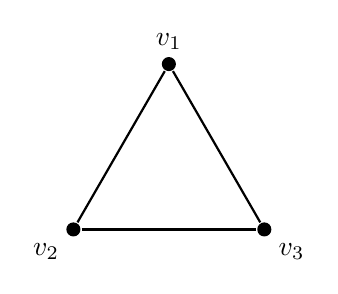
\begin{tikzpicture}[
      vertex/.style={circle, fill=black, inner sep=1.8pt},
      every label/.style={inner sep=2pt},
      thick
    ]
      \node[vertex, label=above:$v_1$] (v1) at (90:1.4)  {};
      \node[vertex, label={[label distance=1pt]below left:$v_2$}]  (v2) at (210:1.4) {};
      \node[vertex, label={[label distance=1pt]below right:$v_3$}] (v3) at (330:1.4) {};
      \draw (v1) -- (v2);
      \draw (v2) -- (v3);
      \draw (v3) -- (v1);
    \end{tikzpicture}
  \end{center}
  Matrice di adiacenza:
  \[
    A(K_3) = J - I = \begin{pmatrix} 0 & 1 & 1 \\ 1 & 0 & 1 \\ 1 & 1 & 0 \end{pmatrix} .
  \]
  Autovalori: $ 2 $ (semplice, autovettore $ (1,1,1)^T $) e $ -1 $ (con molteplicita' $ 2 $).
}

\mlenma{Autovalori di $ J $}{\label{lem:autovalori-J}
  Gli autovalori della matrice $ J \in \mathbb{R}^{p \times p} $ sono:
  \begin{itemize}
    \item $ p $ con molteplicita' $ 1 $ (autovettore $ (1, 1, \ldots, 1)^T $);
    \item $ 0 $ con molteplicita' $ p - 1 $ (autospazio: vettori a somma nulla).
  \end{itemize}
}

\mprop{Autovalori di $ A(K_p) $}{\label{prop:autovalori-Kp}
  Gli autovalori di $ A(K_p) $ sono:
  \begin{itemize}
    \item $ p - 1 $ con molteplicita' $ 1 $;
    \item $ -1 $ con molteplicita' $ p - 1 $.
  \end{itemize}
}
\pf{Dim}{
  $ v \neq 0 $ e' autovettore di $ A(K_p) = J - I $ con autovalore $ \lambda $ sse $ (J - I)v = \lambda v $, sse $ Jv = (\lambda + 1) v $. Quindi gli autovalori di $ A(K_p) $ sono quelli di $ J $ (Lemma~\ref{lem:autovalori-J}) shifted di $ -1 $: $ p \mapsto p - 1 $ e $ 0 \mapsto -1 $, con le stesse molteplicita'.
}

\cor{Cammini chiusi in $ K_p $ basati in un vertice}{\label{cor:cammini-chiusi-Kp}
  Per ogni $ \ell \geq 1 $ e ogni vertice $ v_i $ di $ K_p $:
  \[
    \bigl(A(K_p)^\ell\bigr)_{ii} = \frac{1}{p}\Bigl( (p-1)^\ell + (p-1)\,(-1)^\ell \Bigr) .
  \]
}
\pf{Dim}{
  Per il Corollario~\ref{cor:cammini-chiusi-traccia} il numero totale di cammini chiusi di lunghezza $ \ell $ in $ K_p $ e'
  \[
    f_{K_p}(\ell) = (p-1)^\ell + \underbrace{(-1)^\ell + \cdots + (-1)^\ell}_{p - 1 \text{ volte}} = (p-1)^\ell + (p-1)\,(-1)^\ell .
  \]
  Per simmetria del grafo completo, ogni vertice contribuisce con lo stesso numero di cammini chiusi: basta dividere per $ p $.
}

\osservazione{
  $ \bigl(A(K_p)^\ell\bigr)_{ii} $ coincide con il numero di successioni $ (i_1, i_2, \ldots, i_{\ell+1}) $ con $ i_j \in \{1, \ldots, p\} $, $ i_1 $ fissato, $ i_{j+1} \neq i_j $ per ogni $ j $ e $ i_{\ell+1} = i_1 $: ad ogni passo, su $ K_p $, si puo' andare a uno qualsiasi degli altri $ p - 1 $ vertici.
}

\subsubsection{Cammini non chiusi in $ K_p $: due metodi}

Quanti sono i cammini di lunghezza $ \ell $ in $ K_p $ da $ v_i $ a $ v_j $ con $ j \neq i $?

\paragraph{Primo metodo: totale meno chiusi.}

I cammini di lunghezza $ \ell $ che partono da $ v_i $ sono $ (p-1)^\ell $: ad ogni passo si hanno $ p - 1 $ scelte (uno qualsiasi degli altri vertici). Sottraendo i chiusi (Corollario~\ref{cor:cammini-chiusi-Kp}) si ottiene il numero di cammini non chiusi che partono da $ v_i $, ripartiti uniformemente fra i $ p - 1 $ vertici di arrivo $ v_j \neq v_i $:
\[
  \bigl(A(K_p)^\ell\bigr)_{ij}
    = \frac{1}{p-1}\!\left( (p-1)^\ell - \frac{(p-1)^\ell + (p-1)(-1)^\ell}{p} \right)
    = \frac{(p-1)^\ell - (-1)^\ell}{p} .
\]

\paragraph{Secondo metodo: espansione binomiale di $ (J - I)^\ell $.}

Sviluppiamo $ (J - I)^\ell $ con il binomio di Newton, valido perche' $ I $ e $ J $ commutano:
\[
  (J - I)^\ell = \sum_{k=0}^{\ell} (-1)^{\ell - k} \binom{\ell}{k}\, J^k .
\]

\osservazione{$ J^k = p^{k-1}\, J $ per ogni $ k \geq 1 $. Infatti $ J^2 $ ha entrata $ (i,j) $ uguale a $ \sum_h 1 \cdot 1 = p $, quindi $ J^2 = pJ $; per induzione, $ J^{k+1} = J \cdot J^k = J \cdot p^{k-1} J = p^{k-1}\, J^2 = p^k J $.}

Sostituendo (e isolando il termine $ k = 0 $, cioe' $ J^0 = I $):
\[
  (J - I)^\ell
    = (-1)^\ell I + \sum_{k=1}^{\ell} (-1)^{\ell - k} \binom{\ell}{k}\, p^{k-1}\, J
    = (-1)^\ell I + \frac{1}{p}\!\left( \sum_{k=1}^{\ell} (-1)^{\ell - k} \binom{\ell}{k}\, p^k \right)\! J .
\]
La somma fra parentesi e' $ (p - 1)^\ell - (-1)^\ell $ (binomio di Newton applicato a $ p $ e $ -1 $, con il termine $ k = 0 $ tolto), quindi:
\[
  \boxed{\;(J - I)^\ell = (-1)^\ell\, I + \frac{(p-1)^\ell - (-1)^\ell}{p}\, J\;}
\]
L'entrata $ (i,j) $ vale dunque:
\begin{itemize}
  \item per $ i = j $: $ (-1)^\ell + \frac{(p-1)^\ell - (-1)^\ell}{p} = \frac{(p-1)^\ell + (p-1)(-1)^\ell}{p} $ (coerente con il Corollario~\ref{cor:cammini-chiusi-Kp});
  \item per $ i \neq j $: $ \frac{(p-1)^\ell - (-1)^\ell}{p} $ (coerente con il primo metodo).
\end{itemize}

\osservazione{
  Il secondo metodo e' notevole perche' fornisce la formula chiusa per $ f_G(\ell) $ \textbf{senza conoscere gli autovalori}: si lavora puramente nella sottoalgebra commutativa generata da $ I $ e $ J $.
}

\subsection{Lemma di unicita' per somme di potenze}

\mlenma{Unicita' delle somme di potenze}{\label{lem:somma-potenze-unicita}
  Siano $ \alpha_1, \ldots, \alpha_r, \beta_1, \ldots, \beta_s \in \mathbb{C} \setminus \{0\} $ tali che per ogni $ \ell \in \mathbb{Z}_{\geq 1} $:
  \[
    \alpha_1^\ell + \cdots + \alpha_r^\ell = \beta_1^\ell + \cdots + \beta_s^\ell .
  \]
  Allora $ r = s $ e, a meno di riordinamenti, $ \alpha_i = \beta_i $ per ogni $ i $.
}
\pf{Dim}{
  Moltiplichiamo entrambi i membri per $ x^\ell $ e sommiamo su $ \ell \geq 1 $. A sinistra:
  \[
    \sum_{\ell \geq 1} \bigl(\alpha_1^\ell + \cdots + \alpha_r^\ell\bigr) x^\ell
      = \sum_{i=1}^{r} \sum_{\ell \geq 1} (\alpha_i x)^\ell
      = \sum_{i=1}^{r} \frac{\alpha_i x}{1 - \alpha_i x}\,,
  \]
  usando la serie geometrica $ \sum_{\ell \geq 1} (\gamma x)^\ell = \gamma x / (1 - \gamma x) $. Analogamente a destra. Si ottiene l'identita' di funzioni razionali:
  \[
    \sum_{i=1}^{r} \frac{\alpha_i x}{1 - \alpha_i x} = \sum_{j=1}^{s} \frac{\beta_j x}{1 - \beta_j x}\,. \tag{$\ast$}
  \]
  Sia $ \{\delta_1, \ldots, \delta_q\} $ l'insieme dei valori \textbf{distinti} che compaiono in $ \{\alpha_1, \ldots, \alpha_r\} \cup \{\beta_1, \ldots, \beta_s\} $, e poniamo
  \[
    m_k := \#\{i \mid \alpha_i = \delta_k\}\,, \qquad m'_k := \#\{j \mid \beta_j = \delta_k\}\,.
  \]
  La tesi e' equivalente a $ m_k = m'_k $ per ogni $ k $. Riscrivendo $ (\ast) $:
  \[
    \sum_{k=1}^{q} (m_k - m'_k)\, \frac{\delta_k x}{1 - \delta_k x} = 0\,.
  \]
  Moltiplicando per $ 1 - \delta_k x $ e valutando in $ x = 1/\delta_k $, tutti gli addendi con indice $ \neq k $ si annullano (contengono il fattore $ 1 - \delta_k x $), mentre l'addendo $ k $-esimo da':
  \[
    (m_k - m'_k)\, \delta_k \cdot \tfrac{1}{\delta_k}\, \prod_{j \neq k}\!\left(1 - \tfrac{\delta_j}{\delta_k}\right) = 0\,.
  \]
  Poiche' $ \delta_j \neq \delta_k $ per $ j \neq k $, il produttoria e' non nulla, dunque $ m_k = m'_k $.
}


\section{Spettro di grafi bipartiti}

\dfn{Grafo bipartito}{\label{def:bipartito}
  Un grafo $ G = (V, E, \varphi) $ e' \textit{bipartito} se esiste una partizione $ V = A \sqcup B $ tale che ogni lato di $ G $ ha un estremo in $ A $ e l'altro in $ B $.
}

\ex{$ P_3 $ e' bipartito}{
  Il cammino $ P_3 $ con vertici $ \{v_1, v_2, v_3\} $ e lati $ v_1 v_2, v_2 v_3 $ e' bipartito con $ A = \{v_1, v_3\} $, $ B = \{v_2\} $.
  \begin{center}
    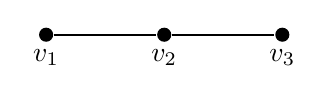
\begin{tikzpicture}[
      vertex/.style={circle, fill=black, inner sep=1.8pt},
      every label/.style={inner sep=2pt},
      thick
    ]
      \node[vertex, label=below:$v_1$] (v1) at (-1.5, 0) {};
      \node[vertex, label=below:$v_2$] (v2) at (0, 0)    {};
      \node[vertex, label=below:$v_3$] (v3) at (1.5, 0)  {};
      \draw (v1) -- (v2) -- (v3);
    \end{tikzpicture}
  \end{center}
  Matrice di adiacenza:
  \[
    A(P_3) = \begin{pmatrix} 0 & 1 & 0 \\ 1 & 0 & 1 \\ 0 & 1 & 0 \end{pmatrix}\,,
  \]
  con autovalori $ \sqrt{2}, 0, -\sqrt{2} $. Osserviamo che $ 0 $ e' autovalore e che lo spettro e' \textbf{simmetrico} rispetto a $ 0 $.
}

\nt{In un grafo bipartito, ogni cammino chiuso ha lunghezza \textbf{pari}: ogni lato attraversa la partizione, quindi un cammino chiuso che ritorna al punto di partenza deve fare un numero pari di attraversamenti. In particolare $ f_G(\ell) = 0 $ per ogni $ \ell $ dispari.}

\mprop{Spettro di un grafo bipartito}{\label{prop:spettro-bipartito}
  Se $ G $ e' bipartito e $ \lambda $ e' autovalore di $ A(G) $, allora anche $ -\lambda $ e' autovalore (con stessa molteplicita').
}

Prima di dimostrarla, richiamiamo lo strumento algebrico chiave.

\dfnc{Funzioni simmetriche elementari e potenze}{\label{def:e-p}
  Per variabili $ x_1, \ldots, x_p $:
  \[
    e_k := \sum_{1 \leq i_1 < i_2 < \cdots < i_k \leq p} x_{i_1} x_{i_2} \cdots x_{i_k}\,, \qquad p_\ell := \sum_{i=1}^{p} x_i^\ell\,,
  \]
  con la convenzione $ e_0 = 1 $.
}

\thm{Formula di Newton}{\label{thm:newton}
  Per ogni $ k \geq 1 $:
  \[
    k\, e_k = \sum_{i=1}^{k} (-1)^{i-1}\, p_i\, e_{k-i}\,.
  \]
}

\pf{Dim della Proposizione~\ref{prop:spettro-bipartito}}{
  Siano $ \lambda_1, \ldots, \lambda_p $ gli autovalori di $ A(G) $ (con molteplicita') e $ \tilde{e}_k := e_k(\lambda_1, \ldots, \lambda_p) $. Il polinomio caratteristico e':
  \[
    p_{A(G)}(x) = \det(x I - A(G)) = \prod_{i=1}^{p} (x - \lambda_i) = x^p - \tilde{e}_1 x^{p-1} + \tilde{e}_2 x^{p-2} - \cdots + (-1)^p \tilde{e}_p\,.
  \]
  Dalla traccia delle potenze, $ p_\ell(\lambda_1, \ldots, \lambda_p) = \sum_i \lambda_i^\ell = \mathrm{Tr}(A(G)^\ell) = f_G(\ell) $. Per la nota sopra, $ G $ bipartito $ \Longrightarrow p_\ell = 0 $ per ogni $ \ell $ dispari.

  \textbf{Per induzione su $ k $ dispari mostriamo $ \tilde{e}_k = 0 $.}
  \begin{itemize}
    \item \textbf{Base ($ k = 1 $):} $ \tilde{e}_1 = p_1 = 0 $.
    \item \textbf{Passo:} sia $ k \geq 3 $ dispari, e supponiamo $ \tilde{e}_1 = \tilde{e}_3 = \cdots = \tilde{e}_{k-2} = 0 $. Per Newton:
    \[
      k\, \tilde{e}_k = \sum_{i=1}^{k} (-1)^{i-1}\, p_i\, \tilde{e}_{k-i}\,.
    \]
    Per ogni $ i $:
    \begin{itemize}
      \item se $ i $ e' dispari, $ p_i = 0 $ (cammini chiusi di lunghezza dispari);
      \item se $ i $ e' pari, $ k - i $ e' dispari (perche' $ k $ dispari), quindi $ \tilde{e}_{k-i} = 0 $ per ipotesi induttiva.
    \end{itemize}
    Ogni addendo si annulla, dunque $ \tilde{e}_k = 0 $.
  \end{itemize}
  Quindi $ \tilde{e}_k = 0 $ per ogni $ k $ dispari, e il polinomio caratteristico contiene solo monomi con la stessa parita' di $ p $:
  \[
    p_{A(G)}(x) = x^p + \tilde{e}_2\, x^{p-2} + \tilde{e}_4\, x^{p-4} + \cdots\,.
  \]
  Sostituendo $ x \mapsto -x $: $ (-x)^{p - 2j} = (-1)^p\, x^{p - 2j} $ per ogni $ j $, da cui
  \[
    p_{A(G)}(-x) = (-1)^p\, p_{A(G)}(x)\,.
  \]
  In particolare $ p_{A(G)}(\lambda) = 0 \Longrightarrow p_{A(G)}(-\lambda) = 0 $: $ -\lambda $ e' autovalore con la stessa molteplicita'.
}

\ex{Esercizio: $ P_n $ con $ n $ dispari}{
  Sia $ P_n $ il cammino con vertici $ v_1, v_2, \ldots, v_n $ e lati $ v_i v_{i+1} $. $ P_n $ e' bipartito (vertici di indice pari/dispari). Per $ n $ dispari, lo spettro e' simmetrico rispetto a $ 0 $: ci sono $ n $ autovalori con $ \lambda \leftrightarrow -\lambda $, ma $ n $ dispari forza l'esistenza di $ \lambda = 0 $ (l'unico fissato dall'involuzione).
}


\section{Il cubo $ n $-dimensionale $ C_n $}

\subsection{Definizione}

\dfn{Cubo $ n $-dimensionale}{\label{def:cubo}
  Sia $ \mathbb{Z}_2 = \{0, 1\} $ con somma modulo $ 2 $. Il \textit{cubo $ n $-dimensionale} (o \textit{ipercubo}) $ C_n $ e' il grafo con:
  \begin{itemize}
    \item vertici $ V(C_n) = \mathbb{Z}_2^n = \underbrace{\mathbb{Z}_2 \times \cdots \times \mathbb{Z}_2}_{n} $;
    \item un lato fra $ u $ e $ v $ se differiscono in \textbf{esattamente una componente}.
  \end{itemize}
  $ C_n $ ha $ 2^n $ vertici e ogni vertice ha grado $ n $.
}

\dfn{Peso di Hamming}{\label{def:hamming}
  Per $ u \in C_n $ si pone
  \[
    \omega(u) := \#\{i \in \{1, \ldots, n\} \mid u_i = 1\}\,,
  \]
  detto \textit{peso di Hamming} di $ u $. Allora c'e' un lato fra $ u $ e $ v $ in $ C_n $ sse $ \omega(u + v) = 1 $.
}

\ex{$ C_2 $ e $ C_3 $}{
  Per $ n = 2 $: quadrato con vertici $ (0,0), (0,1), (1,0), (1,1) $.
  \begin{center}
    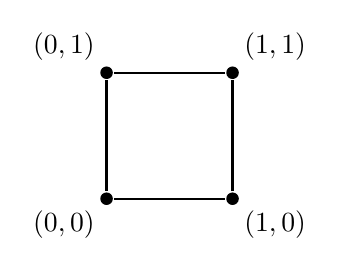
\begin{tikzpicture}[
      vertex/.style={circle, fill=black, inner sep=1.6pt},
      every label/.style={inner sep=2pt},
      thick
    ]
      \node[vertex, label={below left:$(0,0)$}]  (00) at (0, 0)   {};
      \node[vertex, label={below right:$(1,0)$}] (10) at (1.6, 0) {};
      \node[vertex, label={above left:$(0,1)$}]  (01) at (0, 1.6) {};
      \node[vertex, label={above right:$(1,1)$}] (11) at (1.6, 1.6) {};
      \draw (00) -- (10);
      \draw (10) -- (11);
      \draw (11) -- (01);
      \draw (01) -- (00);
    \end{tikzpicture}
  \end{center}
  Per $ n = 3 $: cubo con $ 8 $ vertici.
  \begin{center}
    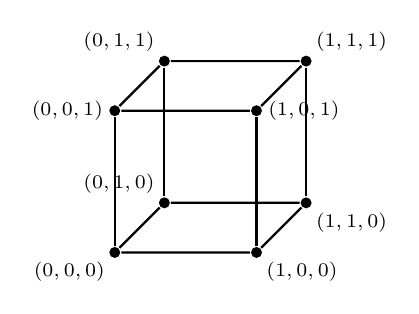
\begin{tikzpicture}[
      vertex/.style={circle, fill=black, inner sep=1.4pt},
      every label/.style={inner sep=1.5pt, font=\scriptsize},
      thick, scale=0.9
    ]
      \node[vertex, label={below left:$(0,0,0)$}]   (000) at (0, 0)   {};
      \node[vertex, label={below right:$(1,0,0)$}]  (100) at (2, 0)   {};
      \node[vertex, label={below right:$(1,1,0)$}]  (110) at (2.7, 0.7) {};
      \node[vertex, label={above left:$(0,1,0)$}]   (010) at (0.7, 0.7) {};
      \node[vertex, label={left:$(0,0,1)$}]         (001) at (0, 2)   {};
      \node[vertex, label={right:$(1,0,1)$}]        (101) at (2, 2)   {};
      \node[vertex, label={above right:$(1,1,1)$}]  (111) at (2.7, 2.7) {};
      \node[vertex, label={above left:$(0,1,1)$}]   (011) at (0.7, 2.7) {};
      \draw (000) -- (100) -- (110) -- (010) -- (000);
      \draw (001) -- (101) -- (111) -- (011) -- (001);
      \draw (000) -- (001);
      \draw (100) -- (101);
      \draw (110) -- (111);
      \draw (010) -- (011);
    \end{tikzpicture}
  \end{center}
}

\nt{$ C_n $ e' bipartito: la partizione e' data dai vertici di peso pari e di peso dispari (un lato cambia esattamente un bit, dunque cambia la parita' del peso). Per la Proposizione~\ref{prop:spettro-bipartito}, lo spettro di $ A(C_n) $ e' simmetrico rispetto a $ 0 $.}

\subsection{Caratteri di $ C_n $}

\dfn{Prodotto scalare in $ \mathbb{Z}_2^n $}{\label{def:prod-Z2}
  Per $ u = (u_1, \ldots, u_n) $ e $ v = (v_1, \ldots, v_n) \in \mathbb{Z}_2^n $:
  \[
    u \cdot v := u_1 v_1 + u_2 v_2 + \cdots + u_n v_n \pmod 2 \in \{0, 1\}\,.
  \]
}

\dfn{Caratteri di $ C_n $}{\label{def:caratteri-cubo}
  Per $ u \in C_n $ definiamo il \textit{carattere} $ \chi_u : C_n \to \mathbb{R} $ come
  \[
    \chi_u(v) := (-1)^{u \cdot v} = \begin{cases} +1 & \text{se } u \cdot v = 0\,, \\ -1 & \text{se } u \cdot v = 1\,. \end{cases}
  \]
}

\mprop{$ \chi_u $ e' un omomorfismo}{\label{prop:caratteri-omom}
  Per ogni $ u \in C_n $, il carattere $ \chi_u $ e' un \textbf{omomorfismo di gruppi} $ (C_n, +) \to (\mathbb{R}^\times, \cdot) $, cioe' per ogni $ v, w \in C_n $:
  \[
    \chi_u(v + w) = \chi_u(v)\, \chi_u(w)\,.
  \]
}
\pf{Dim}{
  Per ogni $ v, w \in C_n $:
  \[
    \chi_u(v + w) = (-1)^{u \cdot (v + w)} = (-1)^{u \cdot v + u \cdot w} = (-1)^{u \cdot v} \cdot (-1)^{u \cdot w} = \chi_u(v)\, \chi_u(w)\,.
  \]
}
\osservazione{
  I $ \chi_u $ con $ u \in C_n $ sono i $ 2^n $ caratteri irriducibili distinti di $ C_n $, dunque sono \textbf{tutti} i caratteri di $ C_n $.
}

\subsection{Spazio delle funzioni e trasformata di Radon}

\dfn{Spazio $ V $ e base canonica}{\label{def:spazio-V-cubo}
  $ V := \{g : C_n \to \mathbb{R}\} $ e' uno spazio vettoriale reale di dimensione $ |C_n| = 2^n $.

  La \textit{base canonica} $ \{\delta_u\}_{u \in C_n} $ e' data da
  \[
    \delta_u(v) := \delta_{u, v} = \begin{cases} 1 & \text{se } u = v\,, \\ 0 & \text{se } u \neq v\,. \end{cases}
  \]
  Ogni $ g \in V $ si scrive in modo unico come $ g = \sum_{u \in C_n} g(u)\, \delta_u $.
}

\dfn{Trasformata di Radon discreta}{\label{def:radon}
  Sia $ P \subseteq C_n $. La \textit{trasformata di Radon discreta} associata a $ P $ e' l'operatore lineare $ \Phi_P : V \to V $ definito da
  \[
    \Phi_P(g)(v) := \sum_{w \in P} g(v + w)\,.
  \]
}

\thm{Diagonalizzazione di $ \Phi_P $}{\label{thm:radon-diag}
  Gli autovettori di $ \Phi_P $ sono i caratteri $ \chi_u $, e l'autovalore associato a $ \chi_u $ e'
  \[
    \lambda_u = \sum_{w \in P} (-1)^{u \cdot w} = \sum_{w \in P} \chi_u(w)\,.
  \]
  La base $ \{\chi_u \mid u \in C_n\} $ diagonalizza \textbf{ogni} $ \Phi_P $.
}

\pf{Dim}{
  Per ogni $ v \in C_n $:
  \[
    \Phi_P(\chi_u)(v) = \sum_{w \in P} \chi_u(v + w) \stackrel{\text{Prop.~\ref{prop:caratteri-omom}}}{=} \sum_{w \in P} \chi_u(v)\, \chi_u(w) = \chi_u(v) \cdot \underbrace{\sum_{w \in P} \chi_u(w)}_{= \lambda_u}\,.
  \]
  Dunque $ \Phi_P(\chi_u) = \lambda_u\, \chi_u $. I $ 2^n $ caratteri $ \chi_u $ sono ortogonali (caratteri irriducibili distinti), dunque linearmente indipendenti, e formano una base di $ V $ che diagonalizza $ \Phi_P $.
}

\nt{
  Quando $ P $ e' l'insieme dei vettori di peso $ 1 $ (cioe' la base canonica $ \{e_1, \ldots, e_n\} $ di $ \mathbb{Z}_2^n $), $ \Phi_P $ coincide con l'\textbf{operatore di adiacenza} di $ C_n $: $ \Phi_P(g)(v) = \sum_{w \sim v} g(w) $.
}

\cor{Autovettori e autovalori di $ A(C_n) $}{\label{cor:spettro-cubo}
  Sia $ P = \{e_1, \ldots, e_n\} $ l'insieme dei vettori di peso $ 1 $ in $ \mathbb{Z}_2^n $, cosicche' $ \Phi_P = A(C_n) $. Per ogni $ u \in \mathbb{Z}_2^n $:
  \begin{itemize}
    \item l'autovettore associato a $ u $, visto come combinazione lineare dei vertici di $ C_n $, e'
    \[
      E_u = \sum_{v \in \mathbb{Z}_2^n} (-1)^{u \cdot v}\, v\,;
    \]
    \item il corrispondente autovalore e'
    \[
      \lambda_u = n - 2\, \omega(u)\,,
    \]
    dove $ \omega(u) $ e' il peso di Hamming di $ u $.
  \end{itemize}
  In particolare $ A(C_n) $ ha autovalore $ n - 2k $ con molteplicita' $ \binom{n}{k} $, per $ k = 0, 1, \ldots, n $. Lo spettro e' simmetrico rispetto a $ 0 $ (\(k \leftrightarrow n - k\)), coerentemente con la Proposizione~\ref{prop:spettro-bipartito}.
}
\pf{Dim}{
  Per ogni $ g \in V $ vale la decomposizione $ g = \sum_v g(v)\, \delta_v $. Applicandola al carattere $ \chi_u $:
  \[
    \chi_u = \sum_{v \in \mathbb{Z}_2^n} \chi_u(v)\, \delta_v = \sum_{v \in \mathbb{Z}_2^n} (-1)^{u \cdot v}\, \delta_v\,.
  \]
  La matrice di $ \Phi_P $ rispetto alla base $ \{\delta_v\} $ coincide con $ A(C_n) $ (rispetto ai vertici $ v $): identificando $ \delta_v \leftrightarrow v $, l'autovettore $ \chi_u $ corrisponde a $ E_u = \sum_v (-1)^{u \cdot v}\, v $.

  Per l'autovalore, dal Teorema~\ref{thm:radon-diag}:
  \[
    \lambda_u = \sum_{w \in P} (-1)^{u \cdot w} = \sum_{i=1}^{n} (-1)^{u \cdot e_i} = \sum_{i=1}^{n} (-1)^{u_i}\,,
  \]
  poiche' $ e_i \cdot u = u_i $. Ci sono $ n - \omega(u) $ indici $ i $ con $ u_i = 0 $ (contributo $ +1 $) e $ \omega(u) $ indici con $ u_i = 1 $ (contributo $ -1 $), quindi
  \[
    \lambda_u = (n - \omega(u)) - \omega(u) = n - 2\, \omega(u)\,.
  \]
  Al variare di $ u \in \mathbb{Z}_2^n $, $ \omega(u) $ assume i valori $ 0, 1, \ldots, n $, e $ \#\{u \mid \omega(u) = k\} = \binom{n}{k} $.
}

% \end{document}
